\section*{Testdesign}
%
Til undersøgelsen bruges robotten, der er illustreret på \autoref{fig:experiment}. Hver testperson bliver stillet overfor robotten fire gange, hvor robotten har hovedet indstillet i fire forskellige positioner. Efter interaktion med robotten skal testpersonerne på en skala evaluere, hvor indbydende de synes robotten er. De fire positioner er illustreret på \autoref{fig:pos1}, \autoref{fig:pos2}, \autoref{fig:pos3} og \autoref{fig:pos4} og har følgende vinkler mellem vandret position:\blankline
%
Position 1: 100 $^{\circ}$\\
Position 2: 65 $^{\circ}$\\
Position 3: 35 $^{\circ}$\\
Position 4: 0 $^{\circ}$\blankline
%
For at balancere stimulipræsentationerne bruges et Latin Square design to gange, hvor testpersonerne bliver udsat for stimuli i følgende rækkefølgen beskrevet i \autoref{tab:Latin}.\blankline
%
\begin{table}[H]
	\centering
	\begin{tabular}{l|c}
		Tetsperson     & Præsentationsrækkefølge af position \\\hline
		Testperson 1   & 1 - 2 - 3 - 4          \\\hline
		Testperson 2   & 2 - 3 - 4 - 1          \\\hline
		Testperson 3   & 3 - 4 - 1 - 2          \\\hline
		Testperson 4   & 4 - 1 - 2 - 3          \\\hline
		Testperson 5   & 1 - 2 - 3 - 4          \\\hline
		Testperson 6   & 2 - 3 - 4 - 1          \\\hline
		Testperson 7   & 3 - 4 - 1 - 2          \\\hline
		Testperson 8   & 4 - 1 - 2 - 3   
	\end{tabular}
	\caption{Præsentationsrækkefølgen af robottens hovedposition.}
	\label{tab:Latin}         
\end{table}
\noindent
%
Testen udføres i kantinen på Fredrik Bajers vej 7, for at simulere et befolket område som eksempelvis en lufthavn. 


%What are your stimuli?

%
\begin{figure}[H]
\centering
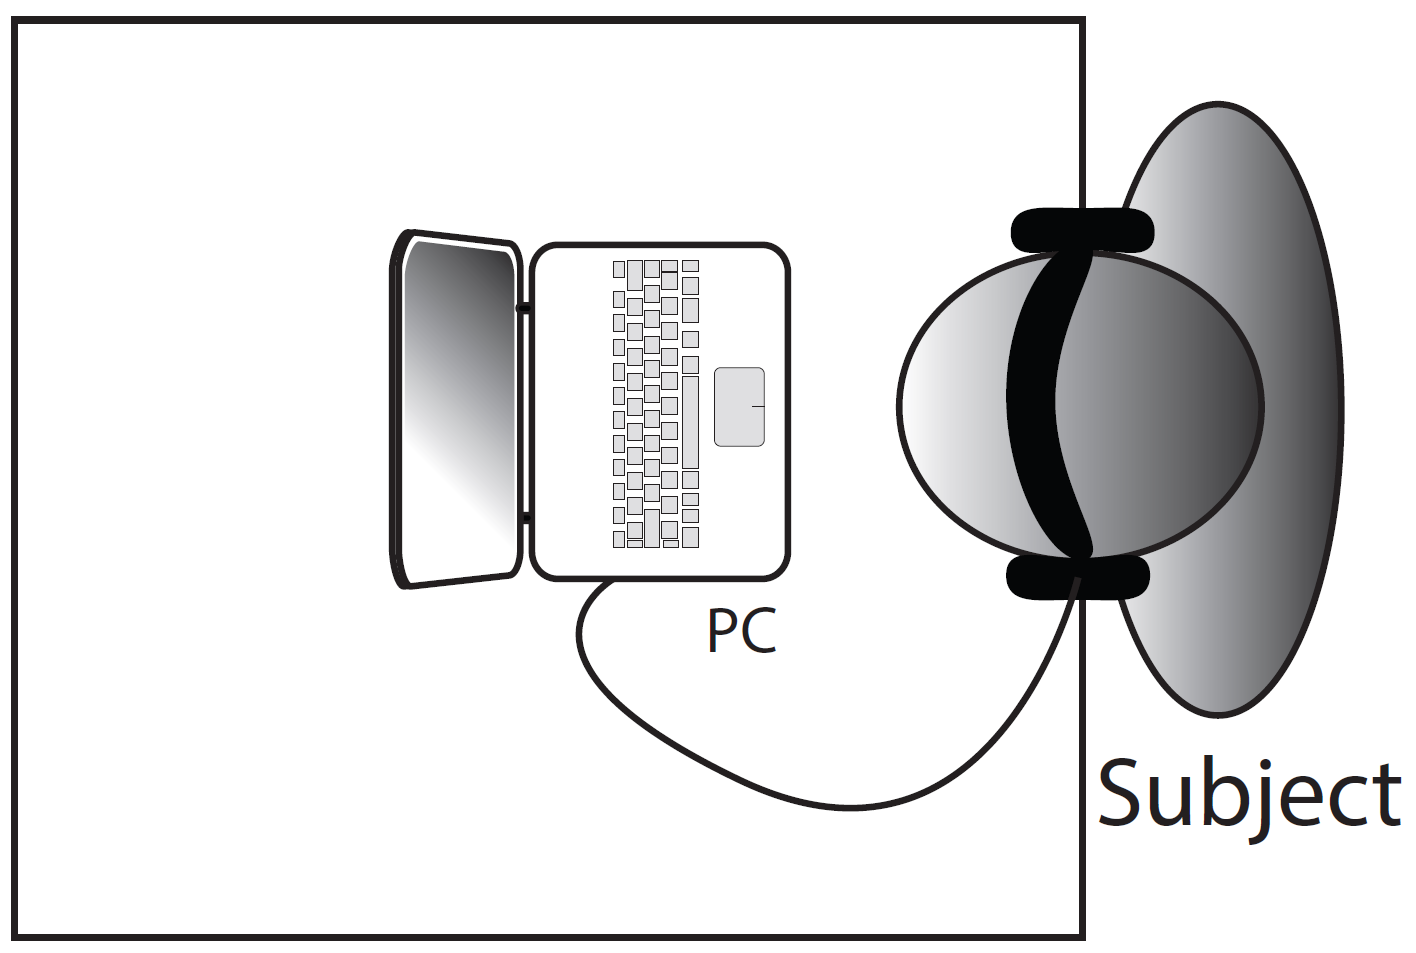
\includegraphics[width = 0.5\textwidth]{Figure/experiment.png} 
\caption{A sketch of the experimental setup.}
\label{fig:experiment}
\end{figure}
%
\subsection*{Design af skalaer}
%
Til testen besluttes det at stille spørgsmålet \textit{"Hvor indbydende synes du robotten er?"}, hvortil testpersonerne kan svare på en \textit{Visual Analog Scale (VAS)}. Skalaen er opstillet med åbne endepunkter og med to ankerpunkter 1,5 cm fra hvert endepunkt. Ved det venstre ankerpunkt er labelen "Slet ikke" givet, mens labelen ved det højre ankerpunkt er "Ekstremt". Ved at ankerpunkterne har de givne labeler kan testpersonen angive hvornår de synes robotten ikke kan blive mere indbydende, og samtidig har de mulighed for at definere den som endnu mere indbydende, hvis næste hovedposition tiltaler dem endnu mere. På denne måde undgås ophobning af svar i endepunkterne.

%Design the scale - argue for the choice and look of the scale.

\subsection*{Test subjects}
%Carry out the scaling experiment on a few subjects (preferably not yourself).
%
Testpersonerne brugt til undersøgelsen er studerende på Aalborg Universitet, herunder studieretningerne jura, kemi-teknologi, fysik og biologi. Testpersonernes alder strækker sig fra 21 år til 34 år med en gennemsnitsalder på 24,6 år.
